% NOTE TO AIP TYPSETERS: TO CONVERT FROM TWO-COL TO PREPRINT, SWITCH
% COMMENTOUT COMMAND FROM A TO B IE. USE:
%
%%\documentclass[prl,twocolumn,showpacs,twocolumngrid,superbib]{revtex4}
%\documentclass[prl,twocolumn,twocolumngrid,superbib]{revtex4}
%\newcommand{\commentoutB}[1]{}
%\newcommand{\commentoutA}[1]{#1}
%
% INSTEAD OF THE FOLLOWING:
%
\newcommand{\commentoutB}[1]{#1}
\newcommand{\commentoutA}[1]{}
%\documentclass[prl,aps,preprint,showpacs,superbib]{revtex4}
\documentclass[prl,aps,preprint,superbib,12pt]{revtex4}

\usepackage{graphicx}
\usepackage{amsfonts}
\usepackage{amsmath}
\usepackage{bm}
\usepackage{alltt}
\usepackage{fancyhdr}
\newcommand{\bms}[1]{{\boldsymbol #1}}
\renewcommand{\thefootnote}{\fnsymbol{footnote}}

%\draft
%\tighten
\pagestyle{fancy}

\begin{document}

\title{Geometry Optimization of Crystals by the Quasi-\\
       Independent Curvilinear Coordinate Approximation}

\author{K\'aroly N\'emeth\footnotemark[1]}
\author{Matt Challacombe}
\author{Christopher J. Tymczak}
\author{Valery Weber}

\affiliation{Theoretical Division,\\ Los Alamos National Laboratory, \\ Los Alamos, NM 87545, USA}

\date{\today}

\begin{abstract}
This paper presents a performance-assessment 
of the recently developed quasi-independent curvilinear coordinate
approximation (QUICCA) method [K. N\'emeth and M. Challacombe,
J. Chem. Phys. {\bf 121}, 2877, (2004)] for the optimization of crystal 
structures. 
We demonstrate that the concept of quasi-independent
curvilinear coordinates is valid also under periodic boundary 
conditions,
and it leads to highly efficient crystal structure optimizations
as illustrated by a series of test calculations. 
The asessment of QUICCA for the optimization of crystal structures
prooves that QUICCA is a generally applicable algorithm
that is highly efficient for the optimization of both isolated 
molecules and crystals while it preserves an unparalleled robustness 
and simplicity of implementation.
\end{abstract}

%\pacs{31.15.-p,31.15.Ne,02.60.Pn, 45.10.Db, 02.40.Hw} 

\maketitle

\footnotetext[1]{\tt KNemeth@LANL.Gov}

\section{Introduction}
Internal coordinates are now routinely used in the optimization of 
molecular structures by most standard quantum chemistry program 
packages. A wealth of experience in geometry optimization justifies
the application of internal coordinates and shows their
superiority as compared to Cartesians. The reason behind the
experience is that internal coordinates exhibit much less
vibrational coupling than Cartesian ones do 
\cite{PPulay69,GFogarasi79,GFogarasi92,PPulay77}.
By recent proposals of Kudin {\it et.al.} \cite{KKudin01} and of
Andzelm {\it et.al.} \cite{JAndzelm01} the foundations of 
internal coordinate
crystal structure optimizations are laid down. These authors
pointed out how to build Wilson's B matrix \cite{EWilson55} 
when periodic boundary conditions are present. They have also
presented a few examples for succesful application of internal 
coordinates for the optimization of crystal structures. It is 
important to note that the paper by Andzelm {\it et.al.}, in our best
understanding, does neither contain the definitions of 
internal coordinate derivatives with respect to lattice parameters,
nor does describe simultaneous internal coordinate relaxation
of both atomic positions and lattice parameters.
The paper by Kudin {\it et.al.} accounts for both of these
features. We find that the construction of Wilson's B matrix
is described in both papers in a less compact, more case-specific 
way, by considering each internal coordinate event by separate 
discussions. This may be instructive but less suitable for
a reader who is interested in quick implementation.
Therefore, we repeat the formulation with the aim of mathematical
compactness that may be better suited for implementation.
Our selection of symmetry unique internal coordinates and treatment
of constraints does also differ from the one proposed by the previous
authors.
More important than these interpretative differences,
our main goal was to
assess the performance of our recently developed robust internal
coordinate optimizer, that is based on the concept of
quasi-independent curvilinear coordinates (QUICCA) \cite{KNemeth04}.
Similar to Baker's test set \cite{JBaker93}, we have set up 
a test set of ten crystal structures that we believe is representative
enough to a very broad range of possible applications. We carry out
geometry optimizations on this test set with the same accuracy
that is used in Baker's test set for isolated molecules.
Test calculations are carried out with both constrained and
relaxed lattice parameters. The results indicate that
QUICCA is generally applicable to both isolated molecule and crystal
structure optimizations, with high efficiency and great robustness,
while preserving an unparalleled simplicity in the implementation.

\section{Lattice summation for Wilson's B matrix}
\subsection{The effective $B$ matrix of the central cell}
Let us consider a three-dimensional crystal with atomic 
Cartesian positions $X$ that extend the range $[-\infty,\infty]$
in all spacial directions. The periodicity of the crystal
is given by the lattice vectors $A$, $B$ and $C$.
For this infinitely large crystal, local internal coordinates ($\phi$) 
can be defined, as usual for isolated molecules. Let us now suppose,
that there is periodicity also in the set of internal coordinates.
This being the case is simply a consequence of applying the 
same rules for the 
construction of internal coordinates everywhere in the crystal.
If this periodicity exists, a unique set of primitive internal 
coordinates, $\phi^{(000)}$ can be defined. Each $i$-th element of this
set, $\phi^{(000)}_{i}$ depends on the Cartesian coordinates of
maximum four atoms: 
\begin{equation}
\phi^{(000)}_{i}=\phi^{(000)}_{i}[
(a_{i1},k_{i1},l_{i1},m_{i1}),
(a_{i2},k_{i2},l_{i2},m_{i2}),
(a_{i3},k_{i3},l_{i3},m_{i3}),
(a_{i4},k_{i4},l_{i4},m_{i4})],
\end{equation}
where $a_{ij}$ ($j=1,2,3,4$) denotes serial numbers of atoms in 
a reference cell, called the 
central cell, and the corresponding $k_{ij}$, $l_{ij}$ and $m_{ij}$ 
denote integer cell indices.
The translationally unique $a_{ij}$ atoms and the 
$k_{ij}$, $l_{ij}$ and $m_{ij}$ 
cell indices together determine
the atoms within the infinite crystal that compose 
the $i$-th internal coordinate of the $\phi^{(000)}$ set. 

It should be noted, that the elementary cell in the
internal coordinate space has a different meaning than what 
the elementary cell in the Cartesian space is. This should
be clear from the fact that the internal coordinate elementary cell 
containes such $\phi^{(000)}_{i}$ coordinates that connect
two or more different Cartesian cells. Furthermore, the internal
coordinate central cell $\phi^{(000)}$ may be located over atoms, 
that are far
from the Cartesian elementary cell. For the sake of simplicity,
we choose the internal coordinate elementary cell to be in maximum
possible overlap with the atoms of the Cartesian elementary cell.

All internal coordinates of the crystal can be retrieved
by applying the same $T_{k_{T}l_{T}m_{T}}=k_{T}A+l_{T}B+m_{T}C$ 
translation vector to the atoms of $\phi^{(000)}$: 
\begin{equation}
\phi^{(k_{T}l_{T}m_{T})}_{i}=\phi^{(000)}_{i}[
(a_{i1},k_{i1}',l_{i1}',m_{i1}'),
(a_{i2},k_{i2}',l_{i2}',m_{i2}'),
(a_{i3},k_{i3}',l_{i3}',m_{i3}'),
(a_{i4},k_{i4}',l_{i4}',m_{i4}')] ,
\end{equation}
where $k_{ij}'=k_{ij}+k_{T}$ and the same holds for the $l$ and $m$ 
cell indices.
$k_{T}$, $l_{T}$ and $m_{T}$ denote arbitrary integers.
The corresponding Cartesian coordinates transform as
\begin{equation}
X^{(k_{ij}+k_{T},l_{ij}+k_{T},m_{ij}+k_{T})}_{a_{ij}} 
= X^{(k_{ij},l_{ij},m_{ij})}_{a_{ij}} + T_{k_{T}l_{T}m_{T}} .
\end{equation} 
All vector quantities here and in the forthcoming derivation
denote row vectors, unless otherwise noted.
Now, let us consider the relationship of an infinitesimally small
Cartesian displacement, $\delta X$ and the corresponding $\delta \phi$
internal coordinate displacement.
Because of the translational symmetry, displacements are the same
in all internal coordinate cells:
\begin{equation}
\delta \phi^{(klm)}_{i} = \delta \phi^{(000)}_{i} 
\end{equation}
for any $i$-th internal coordinate.
The displacements of the Cartesian coordinates, however, do not equal
for different cells: 
\begin{equation} \label{cartdispl}
\delta X^{(klm)}_{a_{ij}} = \delta X^{(000)}_{ij} + k \delta A 
+ l \delta B + m \delta C ,
\end{equation}
with $\delta A$, $\delta B$ and $\delta C$
being the displacements of the lattice vectors. 
The different behaviour of the internal and the Cartesian displacements
reflects the fact, that internal coordinates describe relative
atomic displacements, while Cartesian ones are absolute displacements, 
relative to the Cartesian coordinate axis.

The relationship between the Cartesian and internal coordinate 
displacements can be expressed by Wilson's $B$ matrix:
\begin{equation}
\delta \phi = B \delta X
\end{equation}
where $B$ here has the size of $\infty \times \infty$ and its
elements are given by
\begin{equation}
B_{pq}= \frac{\partial \phi_{p}}{\partial X_{q}} , 
\end{equation}
where $X_{q}$ denotes a single Cartesian coordinate of the set $X$.

It is enough to investigate the relationship of the internal 
coordinates of the central cell and all the Cartesian coordinates,
since all other internal coordinate displacements equal with the 
central cell ones:
\begin{equation} \label{intdispl1}
\delta \phi^{(000)}_{i} = \sum_{q=1}^{\infty} B^{(000)}_{iq} \delta X_{q} .
\end{equation}
Here, $B^{(000)}_{iq}$ denotes elements of the $B$ matrix that refer to
the central internal coordinate cell. All $i$-th internal coordinates
are members of the central internal coordinate cell.
Now, let us further decompose $\delta X_{q}$ and $B^{(000)}_{iq}$ 
to contributions from Cartesian cells:
\begin{equation} \label{latsum1}
\delta \phi^{(000)}_{i} = 
\sum_{j=1}^{4} 
B^{(000)(k_{ij}l_{ij}m_{ij})}_{ia_{ij}} [ \delta X^{(000)}_{a_{ij}} + k_{ij} \delta A + 
l_{ij} \delta B + m_{ij} \delta C ]^{t} ,
\end{equation}
where the superscript $t$ denotes transposition
and $B^{(000)(k_{ij}l_{ij}m_{ij})}_{ia_{ij}}$ is defined by
\begin{equation} 
B^{(000)(k_{ij}l_{ij}m_{ij})}_{ia_{ij}} = \frac{\partial 
\phi^{(000)}_{i}}{\partial X^{(k_{ij}l_{ij}m_{ij})}_{a_{ij}}} .
\end{equation} 
The summation over $j$ goes over those atoms that compose 
the $i$-th internal coordinate. The number of 
these atoms never exceeds four if primitive internal coordinates are used.
In case of more complex internal coordinates that are linear 
combinations of primitive ones, the $B$ matrix of the composite 
internal coordinates will be built
by appropriately transforming the $B$ matrix of the primitives. 
We do not consider this case further in the 
present paper.
Observe that $B^{(000)(k_{ij}l_{ij}m_{ij})}_{ia_{ij}}$ is a 
vector with three components referring to the Cartesian components
of atom $a_{ij}$, {\it and} to the Cartesian components of the
lattice vectors $A$, $B$ and $C$.

Now, let us introduce the matrices 
$B^{(000)(A)}$, $B^{(000)(B)}$ and $B^{(000)(C)}$.
$B^{(000)(A)}$ is constructed by
\begin{equation} \label{matba}
B^{(000)(A)}_{i} = \sum_{j=1}^{4} k_{ij} B^{(000)(k_{ij}l_{ij}m_{ij})}_{ia_{ij}} . 
\end{equation}
$B^{(000)(B)}_{i}$ and $B^{(000)(C)}_{i}$ are given by the same formula 
as $B^{(000)(A)}_{i}$ except that
the multiplicativ factor $k_{ij}$ in Eqn. \ref{matba} is exchanged to 
$l_{ij}$ and $m_{ij}$, respectively. Each of these three matrices
are of the size $N_{i} \times 3$, where $N_{i}$ is the number of
internal coordinates in the central cell $\phi^{000}$.

The displacements of the lattice vectors affect the displacements
of the internal coordinates via the matrices 
$B^{(000)(A)}$, $B^{(000)(B)}$ and $B^{(000)(C)}$.
A certain $j$-th component atom of the $i$-th internal
coordinate gives a nonzero contribution to those of these three
matrices for which it has a nonzero corresponding lattice index.
E.g. if the $j$-th atom is located in the cell $(100)$,
it will contribute only to $B^{(000)(A)}$. It may also happen that
each of the four atoms of an internal coordinate contribute
to all three matrices, $B^{(000)(A)}$, $B^{(000)(B)}$ and $B^{(000)(C)}$,
when all cell-indices of all component-atoms differ from zero.

Thus, Eqn. \ref{latsum1} can be rewritten to
\begin{equation} \label{latsum2}
\delta \phi^{(000)}_{i} = 
B'^{(000)}
\left[
[\oplus_{j=1}^{4} \delta X^{(000)}_{ia_{ij}} ] 
\oplus \delta A 
\oplus \delta B 
\oplus \delta C 
\right]^{t} ,
\end{equation}
where $B'^{(000)}$ denotes the effective $B$ matrix for crystals:
\begin{equation} \label{latsum3}
B'^{(000)}_{i} =
[\oplus_{j=1}^{4}
B^{(000)(k_{ij}l_{ij}m_{ij})}_{ia_{ij}}
] \oplus B^{(000)(A)}_{i} \oplus B^{(000)(B)}_{i} \oplus B^{(000)(C)}_{i} ,
\end{equation}
while the second term of Eqn. \ref{latsum2} 
provides the displacements of the atomic positions
and the lattice vectors.
The description of the effective $B$ matrix, $B'^{(000)}$, 
as provided by Eqn. \ref{latsum2}, deals only with the
nonzero elements of $B'^{(000)}$. However, it should be clear from the
formalism, that
$B'^{(000)}$ has $3N+9$ colums, where $N$ is the number of atoms
in the central cell. This can be seen from the fact, that the subscript 
$a_{ij}$ scans all atoms of the central cell.

We still owe with the determination 
of the values $B^{(000)(k_{ij}l_{ij}m_{ij})}_{ia_{ij}}$.
Whenever these values are to be computed, the absolute Cartesian positions
of any $j$-th atom of the $i$-th internal coordinate are generated, based
on the knowledge of the corresponding translationally unique atom $a_{ij}$
and the cell indices $k_{ij}$, $l_{ij}$ and $m_{ij}$. Once the absolute
Cartesian positions are recovered, $B^{(000)(k_{ij}l_{ij}m_{ij})}_{ia_{ij}}$
is determined exactly as for isolated molecules \cite{EWilson55}. Thus,
the derivation of $B'^{(000)}$ is completed.

\subsection{The effective $A$ matrix of the central cell}

Let us represent the displacements of the Cartesian
positions of the entire crystal, $\delta X$ in a more
compact way now. For each cell with cell indices
$(klm)$ the atomic displacement $\delta X^{(klm)}_{a_{ij}}$
can be decomposed to a translation-free term 
$\delta X^{(000)}_{a_{ij}}$ and to a term $\delta T_{klm}$ that
contains translation:
\begin{equation}
\delta T_{klm} = k \delta A + l \delta B + m \delta C ,
\end{equation}
as it has already been recognized in Eqn. \ref{cartdispl}.
Thus, the total Cartesian displacement can be formulated also as
\begin{equation} \label{newx}
\delta X' = 
\oplus_{k,l,m=-\infty}^{\infty}
\left[ \oplus_{a_{ij}=1}^{N} \delta X^{000}_{a_{ij}} \right]
\oplus
\left[ 
 k \delta A \oplus l \delta B \oplus m \delta C \right] ,
\end{equation}
where the symbol $a_{ij}$ is running over all $N$ atoms
of the central cell. The prime over $X$ distinguishes
the new $X'$ representation from the old $X$ one in the sense
that the old representation had a $3N$ dimensional displacement
vector for each cell, while in the new $X'$ representation
the displacements of the atoms in a cell are represented by
a $3N+9$ dimensional vector.

The $B$ matrix in the new representation, $B'$ can be written
as the direct-sum of $B'^{(klm)(k'l'm')}$ matrices:
\begin{equation}
B' = \oplus_{k,l,m,k',l',m'=-\infty}^{\infty} B'^{(klm)(k'l'm')} ,
\end{equation}
where the cell indices $(klm)$ refer to the internal coordinate
cell, while $(k'l'm')$ refer to the Cartesian cell.

$B'$ should be such, that for any $\delta X'$ displacement vector
the corresponding $\delta \phi^{(klm)}$ internal coordinate
displacements will be the same for any $(klm)$ internal coordinate
cell. And, when multiplying the row-vector of internal coordinate 
displacements $\delta \phi^{(klm)}$ with the generalized inverse
of $B'$, the resulting $\delta X'$ displacements should also
replect the translational symmetry of the crystal.

In order to satisfy these conditions, the offdiagonal 
($(k,l,m)/=(k',l',m')$)
elements of $B'$ must be set to zero:
\begin{equation} \label{kronecker}
B'^{(klm)(k'l'm')} = \delta_{(klm),(k'l'm')} B'^{(klm)} ,
\end{equation}
with $\delta_{(klm),(k'l'm')}$ being one only when the primed
and unprimed cell-indices refer to the same cell, otherwise 
it equals to zero.
$B'^{(klm)}$ must be defined similarly as in Eqn. \ref{latsum2}:
\begin{equation} \label{latsum4}
B'^{(klm)}_{i} =
[\oplus_{j=1}^{4}
B^{(000)(k_{ij}l_{ij}m_{ij})}_{ia_{ij}}
] \oplus B^{(klm)(A)}_{i} \oplus B^{(klm)(B)}_{i} 
\oplus B^{(klm)(C)}_{i} .
\end{equation}
Furthermore, to satisfy the above conditions, 
the matrix $B^{(klm)(A)}$ must take the form
\begin{equation} 
B^{(klm)(A)} = \frac{1}{k} B^{(000)(A)} .
\end{equation}
Similar definitions must hold for $B^{(klm)(B)}$ and
$B^{(klm)(C)}$. 
With these definitions, the $B'$ matrix satisfies all
required conditions.

The advantage of the new $B'$ representation over $B$ is the fact
that $B'$ is block-diagonal in terms of the $(klm)(k'l'm')$
cell-index pairs, while $B$ is not. The block-diagonal representation
of $B'$ easily allowes for the calculation of the generalized
inverse of $B'$, that is called $A'$, while the old representation,
$B$, does not posess this advantage. Clearly, $A'$ can be calculated
by a block-wise inversion of $B'$, while this block-wise inversion
does not apply to $B$.

In order to check the transformation of an internal
coordinate displacement 
$\delta \phi^{(klm)}=\delta \phi^{(000)}$ into 
Cartesian $\delta X'^{(klm)}$
representation, the generalized inverse of $B'{(klm)}$ 
can be written as
\begin{equation}
A'^{(klm)} = D {\left({B'^{(000)}}^t B'^{(000)}\right)}^{-1} D D^{-1} {B'^{(000)}}^t ,
\end{equation}
where $D$ is a diagonal matrix of linear size $3N+9$, with one in the
diagonal positions except for the last $9$ columns, where it takes
$k$, $l$ or $m$ referring to the matrices $B^{(klm)(A)}$, 
$B^{(klm)(B)}$ and $B^{(klm)(C)}$, respectively.
The corresponding $X'^{(klm)}$ displacement is then given by
\begin{equation}
\delta X'^{(klm)} = D \delta \varphi^{(000)} ,
\end{equation}
where $\delta \varphi^{(000)}$ is the same for all $(klm)$ cells and
is given by
\begin{equation}
\delta \varphi^{(000)} = 
{\left({B'^{(000)}}^t B'^{(000)}\right)}^{-1} {B'^{(000)}}^t 
\delta \phi^{(000)}.
\end{equation}
Thus, it is clear, that the dependence of $X'^{(klm)}$ on the
lattice indices $(klm)$ is correct and is in correspondence with
Eqn. \ref{newx}, as required from $A'$. Consequently, $B'$ and $A'$
obey the required symmetry conditions as they should.

Even though previous derivations by Kudin {\it et.al} \cite{KKudin01} 
end up in the same
effective $B$ ($B'^{(000)}$) matrix elements
(after a different derivation process),
we have found it important to justify the use of
$A'^{(000)}$, the generalized inverse of $B'^{(000)}$, as
the effective $A$ matrix of the crystal.

\section{Implementation}

\subsection{Data preparation}
During the process of geometry optimization atomic positions
of the central cell may be folded back to the opposite side of the 
cell, for varios reasons, e.g. because the folded coordinates 
are more convenient for energy and gradient evaluation. The folded
atoms will be translated by a lattice vector.
In geometry optimization this folding may cause a problem. 
Say, we have a 
bond with atoms $A_{1}$ and $A_{2}$, and the cell indices of the
atoms are all zero. The optimizer supposes that this bond existed
during the recent history of the optimization process with exactly
the same lattice indices. If folding happens, in the history
of the length of this bond a jump may occure: the length of the
bond jumps by about the length of a lattice vector. 
One way to avoid such artificial jumps is to keep track
of the history of folding. Another way, which we prefer, is
that Cartesian coordinates of past geometries, after retrieved from 
disk, are compared to a reference geometry (e.g. with the     
very first structure of the optimization process). If the
distance between an atom in the reference geometry and its counterpart
in a retrieved structure is bigger than a lattice vector 
(taken again from the retrieved data set), the retrieved
atomic position will be unfolded, by translating it back 
to the position closest to the reference one.
Then, internal coordinates of the crystal will be identified on the
basis of the unfolded structures, and bonding schemes can easily
be compared and merged if necessary.
In our first paper about the QUICCA optimization algorithm 
\cite{KNemeth04}, we suggested the merging of primary
bonding schemes that come from the retrieved geometries to achieve
a greater stability for larger molecules. Our recent experience tells
us that this merging may not be necessary for achieving
the same stability and efficiency as what was described in our
previous paper \cite{KNemeth04}, though it may be beneficial
for very large molecules. In the present paper,
the internal coordinates used to construct the displaced geometries
were determined solely on the basis of the Cartesian coordinates
provided by the most recent optimization step and the unfolding 
process.

\subsection{Recognition of the internal coordinates}
The Cartesian central cell is replicated so, that all $27$ 
cells with lattice indices between $-1$ and $+1$ are generated.
Even though a smaller replica of 8 cells, with lattice indices
between $0$ and $1$ contains all necessary local internal coordinates,
we prefer to start from the bigger cell, to avoid fragmentation
of molecules at the boundaries of the central cell.
Then, all internal coordinates are recognized in the supercell
by means of the recognition algorithm described in our previous paper
\cite{KNemeth04}, just as for isolated molecules.
Then comes the selection of internal coordinates.
First, all internal coordinates are discarded that do not touch 
the central cell, i.e. do not contain at least one atom with
cell indices $(000)$.
Second, all remaining internal coordinates that have 
negative lattice indices
are translated by the smallest possible translation so that all 
negative lattice indices become zero. If a translated 
internal coordinate
still contains an atom with cell indices $(000)$
the coordinate will be discarded, as it should already have an existing
replica among the non-translated internal ones.
The internal coordinates that have negative
lattice indices and survive the second selection may still
contain translationally equivalent entities. A third selection
filters the translationally unique ones out, by discarding
the internal coordinates that are translated 
by other than a $(001)$ translation vector.

This simple selection scheme allowes for the fast and linear scaling 
recognition of the translationally unique internal coordinates
of the crystal that form the internal coordinate central 
cell $\phi^{(000)}$.

\subsection{The optimizer}
Details of the QUICCA algorithm for geometry optimization are 
described in our previous paper \cite{KNemeth04}. Here we provide 
only a very brief summary of the most important features of the 
optimizer.
QUICCA is based on the realization of the fact, that internal coordinate
gradients show trends during geometry optimization.
These trends can be formalized by weighted curve fitting for each 
individual internal coordinate, over internal coordinate value and 
gradient pairs.
In practice, this curve fitting is most robust with just a line-fit. 
The root of the
fitted curve (line) provides an improved estimate for the minimum
along the internal coordinate. Collectively, these minima determine
the optimization step at the actual geometry.
QUICCA works well, because internal coordinates exhibit  
highly reduced harmonic and anharmonic vibrational coupling, as
compared to Cartesian ones. Furthermore, the fitting process
has an important averaging effect on the vibrational coupling
that also strongly contributes to the success of QUICCA.
A typical fitting process of a gradient curve is illustrated in 
Fig. \ref{iceIh} on a hydrogen bond of the icosahedral (P63/MMC)
ice structure \cite{AGoto90}.

\begin{figure}[h]
\resizebox*{3.5in}{!}{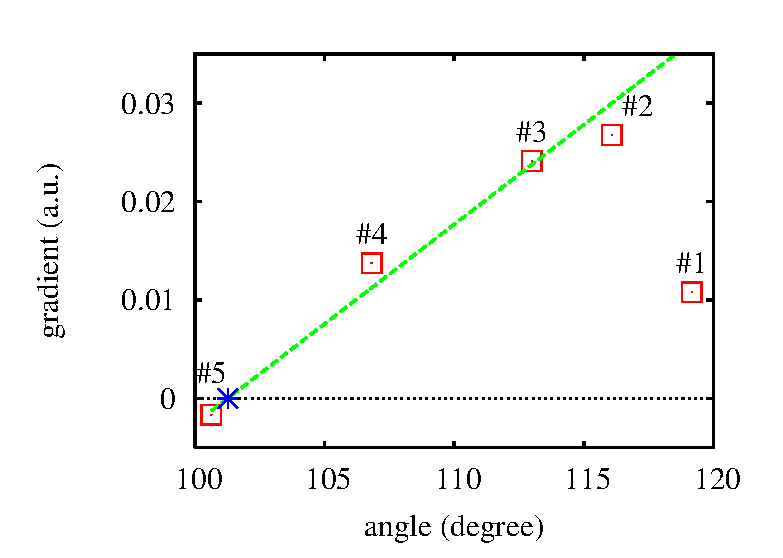
\includegraphics{IceIhfit.eps}}
\caption{
Progression of gradients on a hydrogen bond coordinate
of the icosahedral ice crystal.
Energies and forces have been obtained by the Hartree-Fock
model in STO-3G basis set.
The optimization was started from the crystallographic structure
\cite{AGoto90}.
The numbers in the picture
indicate the sequence of optimization steps. The dashed line represents
a linear fit, the star the predicted location of the minimum.}
\label{iceIh}
\end{figure}

\subsection{Treatment of constraints}
Since the default convergence control of our optimizer
depends only on the magnitude of the largest atomic Cartesian gradient  
vector, the convergence control and the rest of the optimizer
is provided with Cartesian gradients, that do not contain contribution
from the space of constraints. To project out the constraint-space
contribution from the genuine Cartesian gradients, we use the 
projection scheme described in Ref.~\onlinecite{PPulay77}.

In the rest of the treatment of the constraints, we distinguish
the soft and the hard constraints.
Soft constraints approach their required value during the
optimization process and will be set latest at the end of the
optimization. Most internal coordinate constraints are such
in our implementation. Hard constraints are set to their required
value right at the beginning of the optimization process and keep their
value through the entire optimization process. 
Cartesian constraints and lattice constraints are hard constraints 
in our implementation. In the paper by Kudin {\it et.al} \cite{KKudin01}
lattice constraints have been represented by explicite internal
coordinates. This is disadvantageous, since these internal coordinates 
are not local ones and do not refer to chemical entities, such as bond
lengths and bond angles. Consequently, they are much stronger coupled
to the rest of the optimization coordinates as the real local internal 
coordinates.

Our way of treating hard constraints, such as the lattice parameters
is very simple and does not induce extra coupling effects. 
First, those coulumns of the $B$ matrix that refer 
to hard constraints are entirely zeroed. 
The zeroing process in the B matrix reflects the simple fact 
that the variation of any internal coordinate may not contain 
contribution from a Cartesian coordinate or lattice parameter 
that is constrained.

The zeroing of the selected colums of $B$ immediately
ensures that during the iterative back-transformation 
\cite{PPulay77} no displacements occure on hard constraints.
The effect of the zeroing on the gradient transformation is that
internal coordinate gradients will have 
no contribution from 
hard-constrained atoms or lattice parameters.

A simple example to test this constraint-treatment is to optimize water
with, say, one hydrogen atom fixed. The constrained optimization
results exactly in the same optimum bondlengths and angle, 
as the unconstrained optimization, as it should do.

We treat soft constraints in a slightly different way. The rows
of the $B$ matrix that referer to soft-constrained internal coordinates
will not be zeroed. The internal coordinate force on this
coordinates will always be zero, since the Cartesian forces have been
purified from any constraint-space component, as described in the first
paragraph of this subsection. During the iterative back-transformation
the soft-constraints-related rows of the B matrix are needed to 
move the actual value of the soft-constrained coordinate towards
its required value.

The traditional treatment of constraints is described in a review
paper of Pulay \cite{PPulay77}. This traditional treatment
involves the zeroing of the constraint-related columns and rows of the
force constant matrix, but, to the best of our understanding,
it does not involve any zeroing of the columns of the $B$ matrix.
By observing the process of the gradient transformation 
\begin{equation}
g_{i} = g_{c} G_{c}^{-1} B^{t},
\end{equation}
with $g_{c}$ being the constraints-purified Cartesian gradient,
$g_{i}$ the internal coordinate gradient and $G_{c}^{-1}$ 
the generalized inverse of $B^{t}B$, it should be clear,
that even if the same $g_{c}$ vectors enter the process, the two
constraint treatments will result in different internal coordinate 
gradients, $g_{i}$.
Of course, as the optimization proceeds $g_{c}$ and $g_{i}$ will
decrease in both cases and the resulting optimum geometries
should tend towards the same structure.
To the best of our understanding our proposed treatment of constraints
has not been used in the literature of internal coordinate
geometry optimization so far.

If a lattice parameter is constrained, say 
$a=|A|$, the corresponding subspace is projected out from the
columns of the $B'^{(000)(A)}$, $B'^{(000)(B)}$ and $B'^{(000)(C)}$
matrices. To do so, the corresponding Jacobian is needed.

The Jacobian of the lattice parameters can easily be constructed,
as they correspond to streches or bendings between translationally
equivalent atoms. E.g. the lattice parameter $|A|$ can be represented
by a stretching between atom nr. $1$ in the cell $(000)$ and 
atom nr. $1$ in $(100)$. 

The internal coordinates representing
lattice parameters, will have
a non-zero contribution only to the 
$B'^{(000)(A)}$, $B'^{(000)(B)}$ and $B'^{(000)(C)}$
 matrices. Their contribution to $B'^{(000)}$
is exactly zero, which reflects the fact, that no internal
coordinate contributes to the translation or rotation of the
molecule, and thus the vectorial sum of the atomic $B_{i,a_{ij}}$ 
$B$ matrix components should be zero for any $i$-th internal coordinate:
\begin{equation}
\sum_{j=1}^{4} B_{i,a_{ij}} = 0 .
\end{equation}

For $a=|A|$ the corresponding Jacobian is given by 
$\partial a / \partial A$, $\partial a / \partial B$ 
and $\partial a / \partial C$.
If the number of constrained lattice parameters is $N_{r}$,
the corresponding Jacobian, $B_{r}$ is filled into a 
$N_{r} \times 9$ matrix, and the purification of 
$B'^{(000)(A)}$, $B'^{(000)(B)}$ and $B'^{(000)(C)}$
goes like
\begin{equation}
\left[ B'^{(000)(A)} \oplus B'^{(000)(B)} \oplus B'^{(000)(C)} \right]^{\rm pur} =
\left[ B'^{(000)(A)} \oplus B'^{(000)(B)} \oplus B'^{(000)(C)} \right]
\left[ I-B_{r}^{t}(B_{r}B_{r}^{t})^{-1}B_{r} \right] ,
\end{equation}
where $I$ is the $9 \times 9$ identity matrix and the superscript  
``${\rm pur}$'' refers to the result of the purification.

\subsection{Realization}
The crystal structure optimizer has been implemented in the
MondoSCF suite of linear scaling quantum chemistry codes 
\cite{MondoSCF}, in the FORTRAN-90/95 programming language.
Lattice forces have been calculated analytically, as described in 
Ref.~\cite{CJTymczak04LatF}. Note, that all energies and gradients
have been calculated by means of the gamma point approximation,
i.e. there is no band structure calculation in our treatment.

\section{Results and discussion}
\subsection{The test set}
Our test set of crystal structures contains
10 different systems:
Polyacetilene, boron-nitride, diamond, (10,0)carbon-nanotube,
Ice \cite{AGoto90}, Urea \cite{SSwaminathan84}, 
Benzene \cite{GJeffrey87}, Halite, Sulphure, Quartz.
Most of the structures were
taken either from the Inorganic Crystal Stuctures Database
(ICSD) \cite{ICSD} or from Cambridge Crystallographic Data Center
\cite{CCDC} and the translationally unique positions were
generated using Mercury \cite{Mercury}. 
A brief description follows to provide data for the reproduction
of input structures in case they cannot be found
in the above mentioned data bases. 

\subsubsection{Polyacetilene}


\bibliography{../../Bib/mondo_new}
\end{document}
